\section{System-API}
\label{chapAPI}
Die System-API dient als Schnittstelle von Anwendungen und dem Kernel selbst und erlauben einer Anwendung bestimmte Befehle oder Funktionen im Kernel auszuführen. In diesem Kapitel wird sowohl der Ablauf, als auch der Aufbau der System-API genauer erläutert.

\subsection{Ablauf eines \textit{System Calls}}
Der eigentliche Zugriff auf das System über die System-API wird auch als \textit{System Call} bezeichnet. In Listing \ref{fig:Sequencediagram-systemcall} ist ersichtlich wie der grundsätzliche Ablauf eines \textit{System Calls} implementiert wurde. Diesbezüglich bemerkenswert ist, dass einer Anwendung eine intuitive System-API zur Verfügung steht, welche in einer \textit{Library} ausimplementiert ist. Diese Implementierung, welche grundsätzlich noch im \textit{User Mode} ausgeführt wird, erstellt aus dem Funktionsaufruf ein fest definiertes Datenobjekt, welches auf dem \textit{Stack} abgelegt wird. Über einen \textit{Software Interrupt} wird schließlich in den \textit{System Mode} gewechselt und das Datenobjekt in der Kernelimplementierung der System-API wieder interpretiert. Die Werte des Datenobjekts werden schließlich entsprechend der Rückgabewerte des \textit{System Calls} geändert und mittels der Kontextwiederherstellung zum \textit{User Mode} gewechselt. Hier werden durch die \textit{Library}-Implementierung die neuen Daten aus dem Datenpaket extrahiert und als Rückgabewert für die System-API-Funktion verwendet.

\begin{figure}[H]
	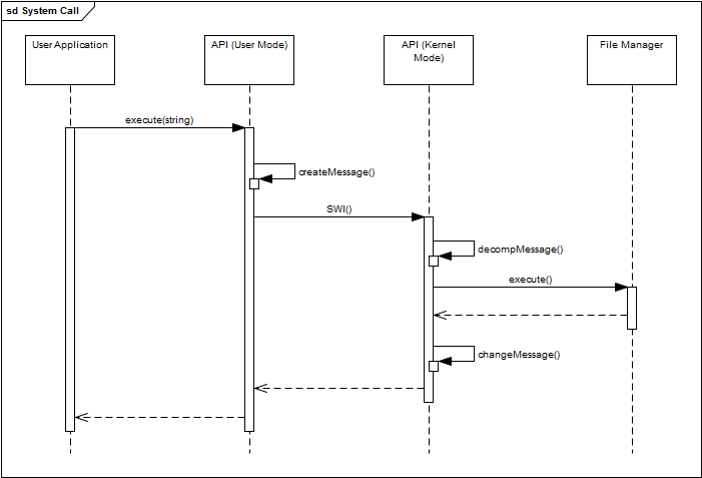
\includegraphics[scale=0.60]{chapters/systemapi/figures/systemcall-sequence-diagram}
	\caption{Sequenzdiagramm eines Systemcalls}
	\label{fig:Sequencediagram-systemcall}
\end{figure}

Der Aufbau eines Datenobjekts welcher zum Datenaustausch zwischen \textit{User Mode} und \textit{System Mode} verwendet wird ist in Listing \ref{systemcall-datapackage} abgebildet.

\lstinputlisting[language=C, caption=Aufbau eines Systemcall Datenpakets, captionpos=b, label=systemcall-datapackage]{chapters/systemapi/codefiles/datapackage.c}

\subsection{Implementierte Funktionen}
Im Folgenden ist eine vollständige Auflistung der implementierten System-API ersichtlich. Es wurde darauf geachtet, die einzelnen Funktionen in verschiedenen \textit{Header}-Dateien zu deklarieren, um eine möglichst \textit{POSIX}-konforme Realisierung zu gewährleisten. Auf die Auflistung der Parameter wurde teilweise aus Komplexitätsgründen verzichtet.

\begin{itemize}
\item \textit{Header}-Datei \textit{devices.h}
\begin{itemize}
\item \texttt{open\_device(char* device)}
\item \texttt{close\_device(int handle)}
\item \texttt{ioctl\_device(int handle, ...)}
\item \texttt{write\_device(int handle, ...)}
\end{itemize}

\item \textit{Header}-Datei \textit{filesystem.h}
\begin{itemize}
\item \texttt{read\_cwd(...)}
\item \texttt{read\_file(char* name, int start, int len, ...)}
\item \texttt{read\_directory(...)}
\item \texttt{set\_cwd(char* directory)}
\end{itemize}

\item \textit{Header}-Datei \textit{ipc.h}
\begin{itemize}
\item \texttt{open\_ipc\_channel(char* namespace)}
\item \texttt{close\_ipc\_channel(char* namespace)}
\item \texttt{send\_ipc\_message(...)}
\item \texttt{has\_ipc\_message(char* namespace)}
\item \texttt{get\_next\_ipc\_message(...)}
\item \texttt{list\_ipc\_channels(...)}
\end{itemize}

\item \textit{Header}-Datei \textit{process.h}
\begin{itemize}
\item \texttt{get\_process\_count()}
\item \texttt{read\_processes(processInfoAPI\_t* buf, int len)}
\item \texttt{kill\_process(int id)}

\end{itemize}

\item \textit{Header}-Datei \textit{system.h}
\begin{itemize}
\item \texttt{execute(char* command)}
\item \texttt{yield()}
\item \texttt{exit(int code)}
\item \texttt{sleep(unsigned int millis)}
\item \texttt{print(...)}\footnote{Diese Funktion ist lediglich eine Hilfsfunktion für das \textit{Retargetting} von \texttt{printf(...)}}
\item \texttt{uptime()}
\end{itemize}

\end{itemize}

\pagebreak 
